\chapter{Our Approach}
\label{chap:approach}

\section{Overview}

This chapter describes the taken approach for generating images from a natural language description. In this approach, we split the task into two by generating a scene graph from the description and subsequently using the scene graph to generate the image. The image generation pipeline is depicted in \Cref{fig:pipeline} below.

\begin{figure}[h]
    \resizebox{\textwidth}{!}{
    \begin{tikzpicture}[node distance=3cm]
     
        \draw (-80bp,75bp) node[text width=7cm]{\Large \say{A duck is swimming in a pond. A tree is next to the pond.}};
    
        \draw [->] (25bp,75bp) -- (55bp,75bp);
    
        \draw (71.0bp,46.5bp) -- (71.0bp,144.5bp) -- (274.0bp,144.5bp) -- (274.0bp,46.5bp) -- cycle;
        \draw (172.5bp,133.0bp) node {\Large group};
        \draw [->] (133.19bp,92.3bp) .. controls (152.83bp,90.652bp) and (179.94bp,88.375bp)  .. (211.85bp,85.696bp);
        \draw (172.5bp,96.0bp) node {\large IN};
        \draw [->] (133.19bp,31.497bp) .. controls (153.19bp,41.417bp) and (180.93bp,55.183bp)  .. (211.85bp,70.525bp);
        \draw (172.5bp,60.0bp) node {\large NEXT TO};
        \draw (79.0bp,76.5bp) -- (79.0bp,112.5bp) -- (133.0bp,112.5bp) -- (133.0bp,76.5bp) -- cycle;
        \draw (106.0bp,94.5bp) node {\Large duck};
        \draw (212.0bp,65.5bp) -- (212.0bp,101.5bp) -- (266.0bp,101.5bp) -- (266.0bp,65.5bp) -- cycle;
        \draw (239.0bp,83.5bp) node {\Large pond};
        \draw (79.0bp,0.5bp) -- (79.0bp,36.5bp) -- (133.0bp,36.5bp) -- (133.0bp,0.5bp) -- cycle;
        \draw (106.0bp,18.5bp) node {\Large tree};
        
        \draw [->] (285bp,75bp) -- (315bp,75bp);
        
        \draw (425bp, 75bp) node{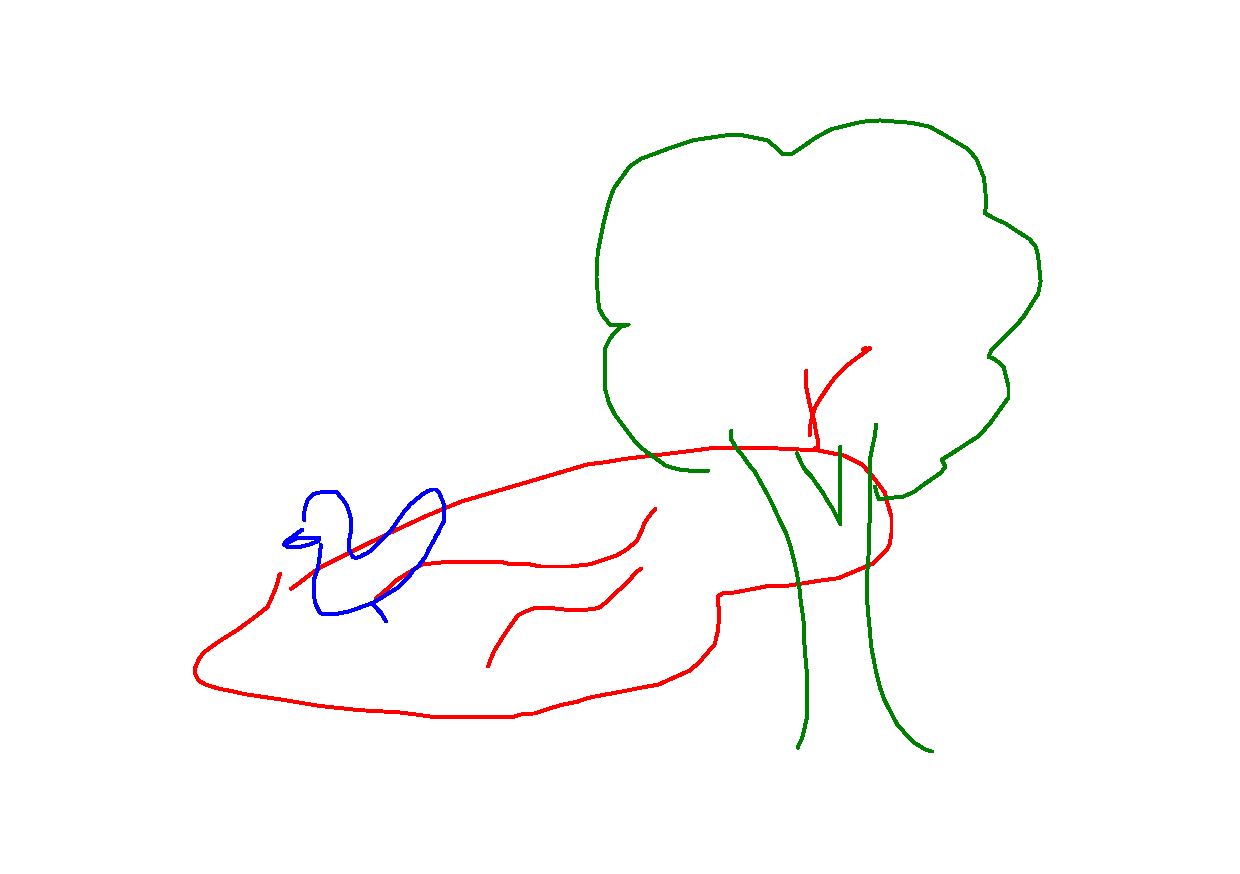
\includegraphics[width=200bp,trim=80 0 80 0,clip]{figures/duck_pond_tree_scene.pdf}};
    
    \end{tikzpicture}
    }
\end{figure}


\section{Description Processing}
\label{sec:description_processing}

The scene graph is a structure that represents the mutual relations between objects in the scene. Our approach uses syntactic analysis as a shallow semantics parser. Using syntactic analysis, we can extract relations between individual words in the sentences and use these relations to build a scene graph. In the following sections, we discuss the limitations of this approach and present a rule-based algorithm for transforming the syntactic dependency tree into a scene graph.

\subsection{Limitations}

In some cases, the syntactic structure of a sentence does not contain all the necessary semantic information to construct a corresponding scene graph. For instance, consider the two sentences \say{A man in a car is on the seat} and \say{A man in a car is on the road}. These two sentences have the same syntactic structure (\Cref{fig:dependency_trees:1}). In the first sentence, semantically, the preposition \say{on} describes the relation between the man and the seat. However, in the second sentence, the same preposition puts into relation the whole car (including the man) and the road. We do not attempt to address this problem in our thesis and accept it as a limitation of our approach.

\begin{figure}[ht]
    \centering
    \begin{subfigure}{0.4\textwidth}
        \centering
        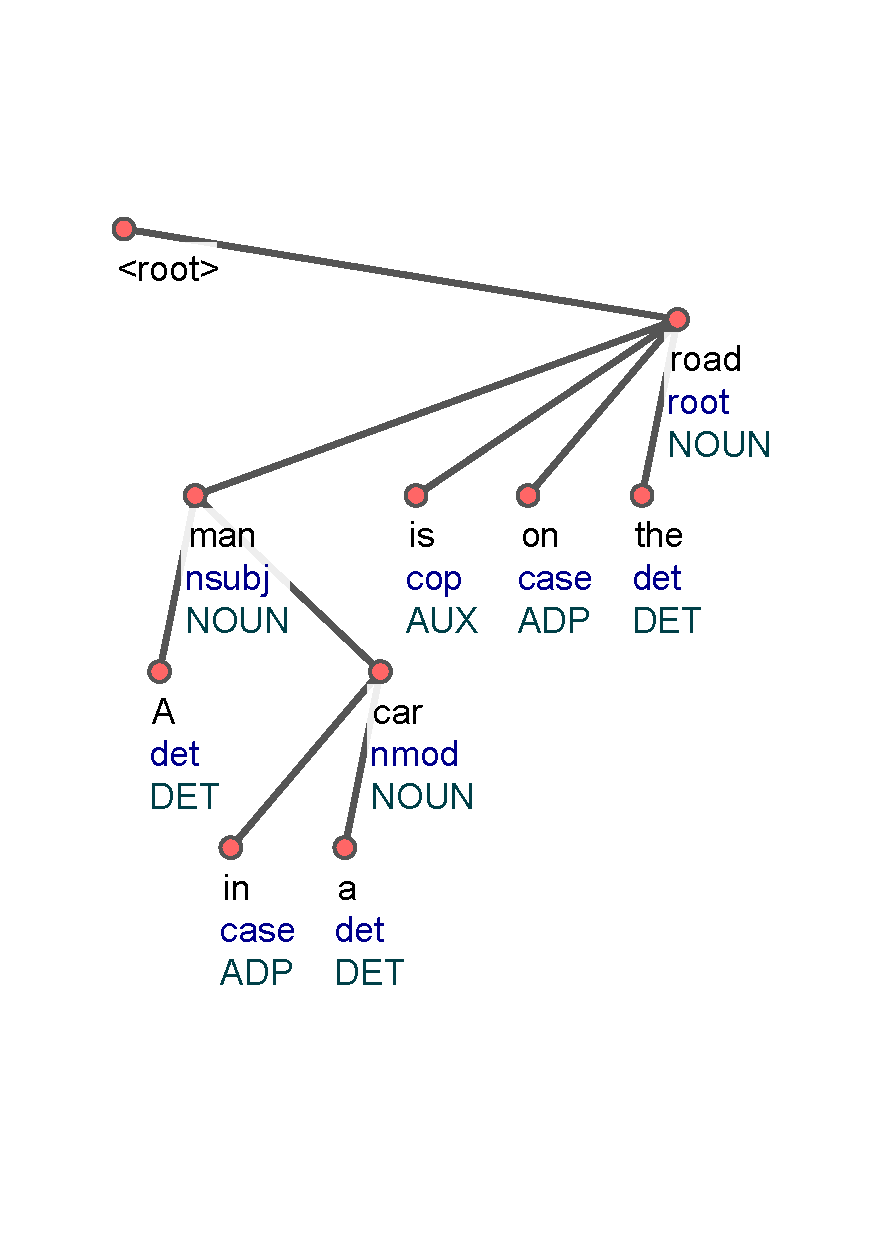
\includegraphics[width=\textwidth,trim=20 120 20 100,clip]{figures/tree_1.pdf}
    \end{subfigure}
    \hskip 25pt
    \begin{subfigure}{0.4\textwidth}
        \centering
        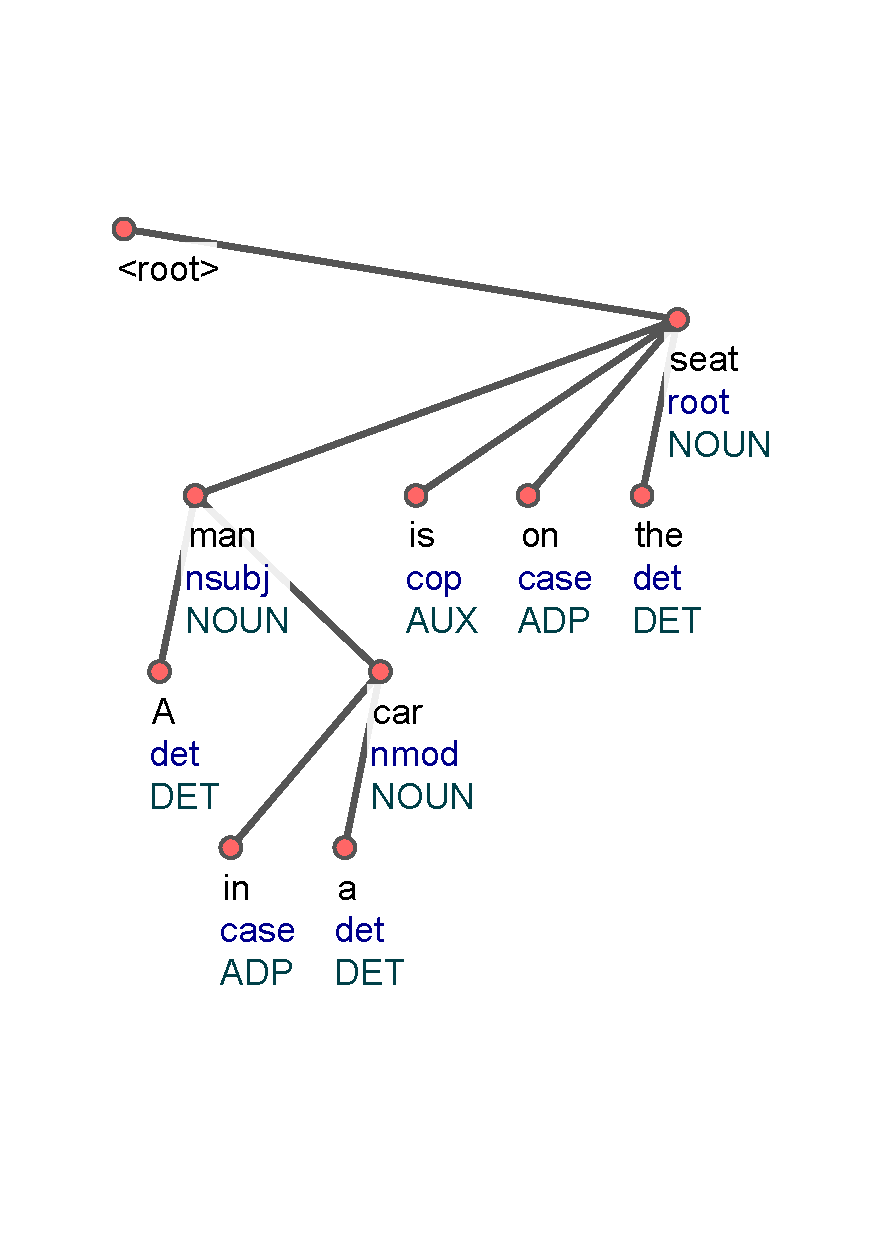
\includegraphics[width=\textwidth,trim=20 120 20 100,clip]{figures/tree_2.pdf}
    \end{subfigure}
    \caption[Sentences with the same syntactic structure but different semantics]{Sentences with the same syntactic structure but different semantics.\protect\footref{footnote:udpipe}}
    \label{fig:dependency_trees:1}
\end{figure}

\subsection{Dependency Tree Parsing}

Our approach uses a tree traversal algorithm to extract the objects and relations from the description. This algorithm is applied to a syntactic dependency tree of the description. In our implementation, we use UDPipe \citep{straka2018udpipe} to obtain the dependency trees in \emph{Universal Dependencies version 2} \citep{nivre2020universal} \emph{CoNLL-U} format. The algorithm uses some properties of this format. The implementation is further discussed in \fullref{chap:impl_details}.

\medskip

The goal of the algorithm is to identify the relations between objects in the dependency tree as semantic subject-predicate-object triples. Note that, unless stated otherwise, whenever we refer to subject-predicate-object triples, we refer to the semantic meaning, not syntactic. The algorithm searches for paths in the dependency tree that contain two nouns --- representing the subject and the object --- and an adposition representing the predicate. The algorithm can be extended to support verb predicates as well; However, we decided to restrict ourselves to position adpositions. The algorithm traverses the dependency tree in a depth-first manner, processing the nodes from left to right. While it traverses the tree, it maintains a stack of created objects. These objects are created when the algorithm opens a node with a noun. When a node with an adposition is opened, we create a new relation by taking two objects from the object stack.

\medskip

To allow relations between groups of objects, we replace the object stack with an entity stack. An entity is an abstraction of objects and groups of objects. We keep track of how many objects were created in each subtree.  If it is more than one, these objects are removed from the stack to form a group that is added to the top of the stack. Therefore, we can create a relation including a group of objects.

\medskip

Complex adpositions --- adpositions that consist of two or more words --- are concatenated into the rightmost dependency tree node. The algorithm distinguishes three complex adposition types of form: 
\begin{enumerate}
	\item adposition-adposition -- e.g. inside of
	\item adposition-noun-adposition -- e.g. in front of
    \item adverb/adjective-adposition -- e.g. next to
\end{enumerate}
A relation corresponding to the complex adposition is created in the last node; i.e., in the case of \emph{in front of} adposition, dependency tree nodes corresponding to the first two words, \emph{in} and \emph{front}, are skipped.

\medskip

Similarly, compound nouns such as paper clip, light bulb, pickup truck, and others need to be joined to create only one object. The compound nouns are identified by the \emph{Universal Dependency} \citep{nivre2020universal} relation -- \verb|compound|.

\begin{figure}[ht]
    \centering
    \begin{subfigure}{0.5\textwidth}
        \centering
        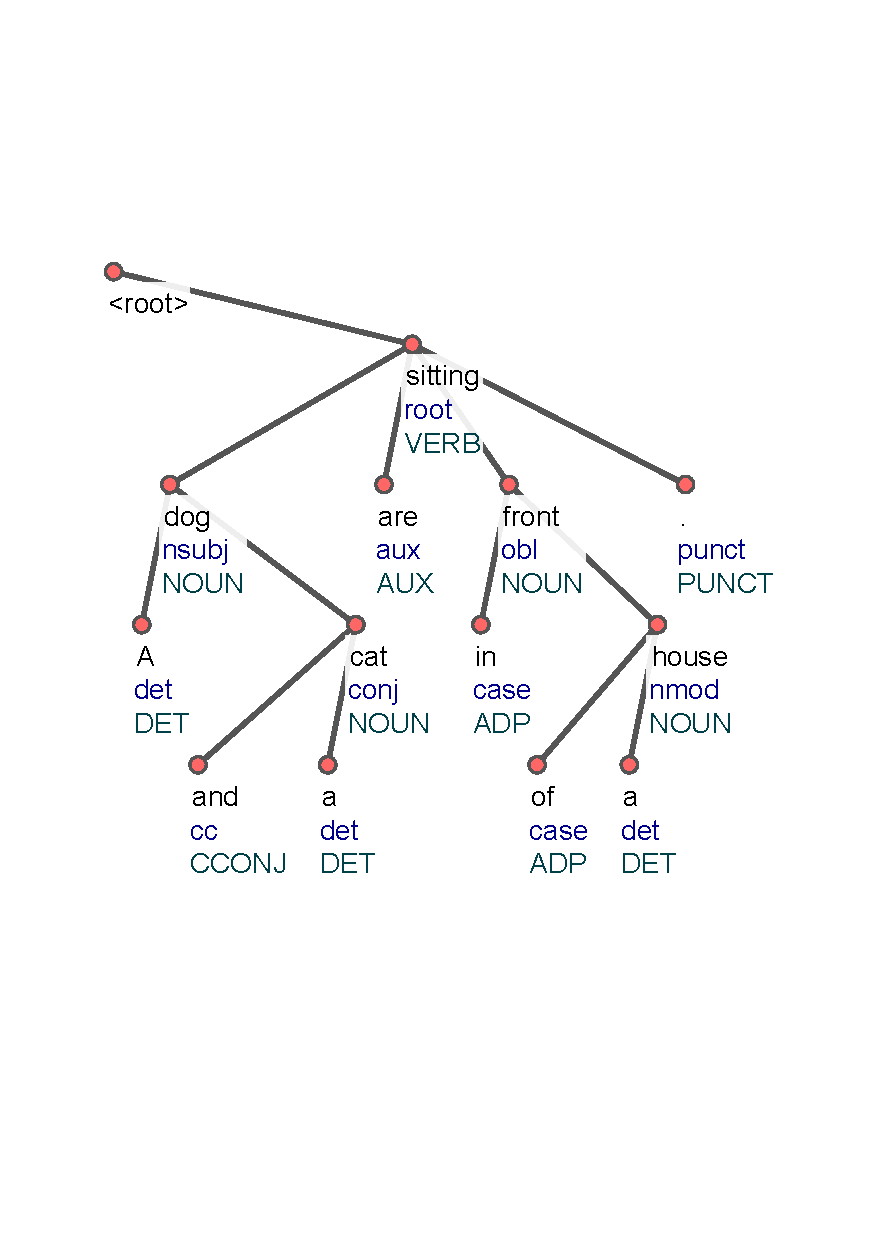
\includegraphics[width=\textwidth,trim=40 160 40 120,clip]{figures/dog_and_cat_in_front_of_house.pdf}
    \end{subfigure}
    \caption[Dependency tree of the example descripton]{Dependency tree of the example descripton.\protect\footref{footnote:udpipe}}
    \label{fig:dependency_trees:2}
\end{figure}
\addtocounter{footnote}{1}
\footnotetext{Dependency tree illustrations were generated using UDPipe LINDAT service \url{https://lindat.mff.cuni.cz/services/udpipe/}. \label{footnote:udpipe}}

\medskip

To illustrate the algorithm, consider the following description: \say{A dog and a cat are sitting in front of a house.}  \Cref{fig:dependency_trees:2} shows the syntactic tree corresponding to the description. The nodes of interest are those corresponding to words \emph{dog}, \emph{cat}, \emph{in}, \emph{front}, \emph{of}, and \emph{house}. The nodes are opened and closed by the depth-first algorithm in this order:


\begin{enumerate}
    \item open \emph{dog}
    \item open \emph{cat}
    \item close \emph{cat}
    \item close \emph{dog}
    \item open \emph{front}
    \item open \emph{in}
    \item close \emph{in}
    \item open \emph{house}
    \item open \emph{of}
    \item close \emph{of}
    \item close \emph{house}
    \item close \emph{front}
\end{enumerate}

The first two steps create new objects and put them on top of the entity stack. In the third step, the node corresponding to the \emph{cat} is closed, but there are no other entities above the cat on the stack; therefore, the stack remains intact. However, when the \emph{dog} node is closed, there is one object on the stack above -- the \emph{cat}. The two objects are therefore taken from the stack merged into a group. Next, the \emph{front} node is opened, which is skipped because it is a part of a complex adposition. The same applies for the \emph{in} node. Opening the \emph{house} node adds a new object to the entity stack. The stack now contains two entities -- The group and the house on top. In the next step, the node \emph{of} is opened. This word is the last part of the complex adposition \emph{in front of} which means that a new relation is created. A relation between the \emph{house} and the group of two objects -- the \emph{dog} and the \emph{cat}.

\section{Composing a Scene}
\label{sec:composing_scene}

The next step in our approach is composing a scene from the scene graph. The scene graph can be viewed as a set of constraints on objects and their positions in the scene. We will use the term \emph{scene composition} as a process of determining the size and position of each object in the scene. Methods used for composing a scene that satisfies the constraints are presented later in this section.

\subsection{Scene Graph Notation}
\label{sec:scene_graph_notation}

A scene graph is a directed graph with labelled edges which describes a particular scene. Each vertex corresponds to an object in the scene. Edges and their labels represent relations between the objects. Throughout this chapter, we will use the following notation for the relation "object $a$ is in relation $p$ with object $b$":
\begin{align}
    a \xrightarrow{p} b
\end{align}
For instance, $dog \xrightarrow{under} tree$ or $book \xrightarrow{on} table$. We will also refer to $a$, $b$, and $p$ as subject, object, and predicate, respectively.

\subsection{Determining the Object's Position}

To compose a scene, we need to determine where to put each object. Object positions have to satisfy the constraints given by the scene graph. In this section, we attempt to formally define the constraints and propose methods for creating and satisfying these constraints. 

\subsection{Positional Constraints}
\label{sec:constraints}

We can think of the object positions as $x$ and $y$ coordinates on a canvas. Thus, we can define the positional constraints as a function of points in the two-dimensional plane with two possible outcomes: $1$ if the constraint is satisfied and $0$ if it is not satisfied. We will denote a constraint function corresponding to a relation $a \xrightarrow{p} b$ as $C_{a,b}^p$. The constraint function is then defined as: 
\begin{align}
    C_{a,b}^p\colon \mathbb{R}^2 \rightarrow \{0, 1\}
    \label{constraint_function}
\end{align}

Suppose we have a constraint function for each relation in the scene graph. Placing an object $a$ within a scene means finding point $(x_a, y_a)$ such that \Cref{math:satisfied} holds for every object $b_i$ which is in relation $a \xrightarrow{p_i} b_i$.
\begin{align}
\label{math:satisfied}
C_{a,b_i}^{p_i}(x_a, y_a) = 1
\end{align}
However, such a point may not exist. Its existence depends on the constraint functions. Therefore, we may accept positions that satisfy a certain portion of the constraints, not necessarily all of them. The approach described in this thesis uses a Monte Carlo algorithm to find a point that satisfies the most constraints on an object. 

\medskip

The Monte Carlo algorithm generates $N$ random normally distributed points $(x_0, y_0), \dots , (x_N, y_N); x_i \sim \mathcal{N}(x_b, w_b), y_i \sim \mathcal{N}(y_b, h_b)$ where $(x_b, y_b)$ and $(w_b, h_b)$ denote the centre of the object and size of object $b$ respectively. Each of the points is tested using all constraint functions associated with objects $a$ and $b$. The first point that satisfies the largest number of constraints is designated as the position of object $a$. This algorithm requires prior knowledge of the position of object b, which requires the existence of topological ordering of the scene graph. 

\subsection{Rule-Based Constraints}
\label{sec:rule_based_constraints}

In the first approach, we define 5 elementary constraint functions and combine these functions to define constraints for selected adpositions. The five constraint functions are:
\begin{enumerate}
    \item \emph{On} constraint -- Tests whether a point is near the top of the object to which the constraint relates. 
    \item \emph{Side} constraint -- Defines a half-plane; all points in the half-plane satisfy the constraint.
    \item \emph{Box} constraint -- Tests whether a point lies within a box.
    \item \emph{Inside} constraint -- Treats the object it relates to as a polygon. A point satisfies this constraint if it lies inside the polygon.
    \item \emph{Disjunction} constraint -- A composite constraint that encapsulates two or more other constraints. The constraint is satisfied if at least one of the encapsulated constraints is satisfied.
\end{enumerate}

\begin{table}[ht]
    \small
    \centering
    \begin{threeparttable}
        \begin{tabular}{p{0.2\linewidth}|p{0.7\linewidth}}
            \textbf{Adposition} & \textbf{Elementary constraint} \\
            \hline \hline
            \emph{in}       &  \emph{Inside} constraint \\
            \hline
            \emph{inside}    & \emph{Inside} constraint \\
            \hline
            \emph{inside of} & \emph{Inside} constraint \\
            \hline
            \emph{on}        & \emph{On} constraint \\
            \hline
            \emph{under}     & \emph{Side} constraint \\
            \hline
            \emph{below}     & \emph{Side} constraint \\
            \hline
            \emph{above}    & \emph{Side} constraint \\
            \hline
            \emph{behind}    & \emph{Box} constraint \\
            \hline
            \emph{in front of} & \emph{Box} constraint \\
            \hline
            \emph{next to} & \emph{Disjuction} constraint (containing two \emph{side} constraints)
        \end{tabular}
    \end{threeparttable}
    \caption[Rule-based constraints]{Rule-based constraints.}
    \label{tab:rule_based_constraints}
\end{table}

Using these elementary constraints we define constraint functions for a small set of adpositions -- \emph{in}, \emph{inside}, \emph{inside of}, \emph{on}, \emph{under}, \emph{below}, \emph{above}, \emph{behind}, \emph{in front of}, and \emph{next to}. \Cref{tab:rule_based_constraints} shows which elementary constraints are used to define the constraints for the listed adpositions. \Cref{sec:constraints_impl} describes how each of the elementary constraints is implemented and provides details on how are these constraints combined. 

\begin{figure}[ht]
    \centering
    \begin{subfigure}{0.45\textwidth}
        \centering
        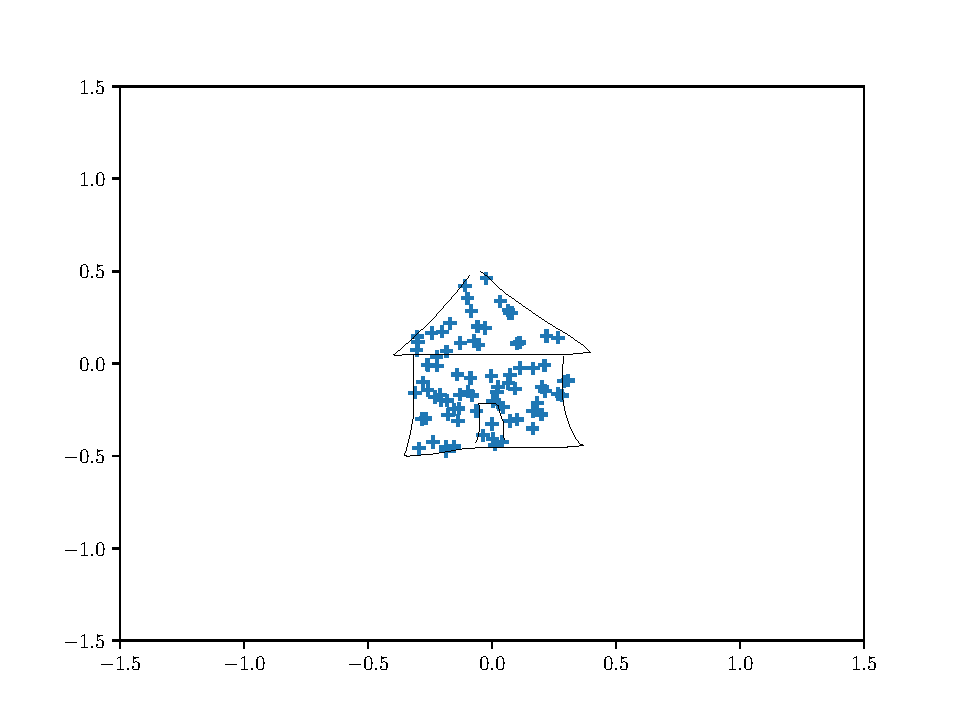
\includegraphics[width=\textwidth]{figures/rule_in_house.pdf}
    \end{subfigure}
    \begin{subfigure}{0.45\textwidth}
        \centering
        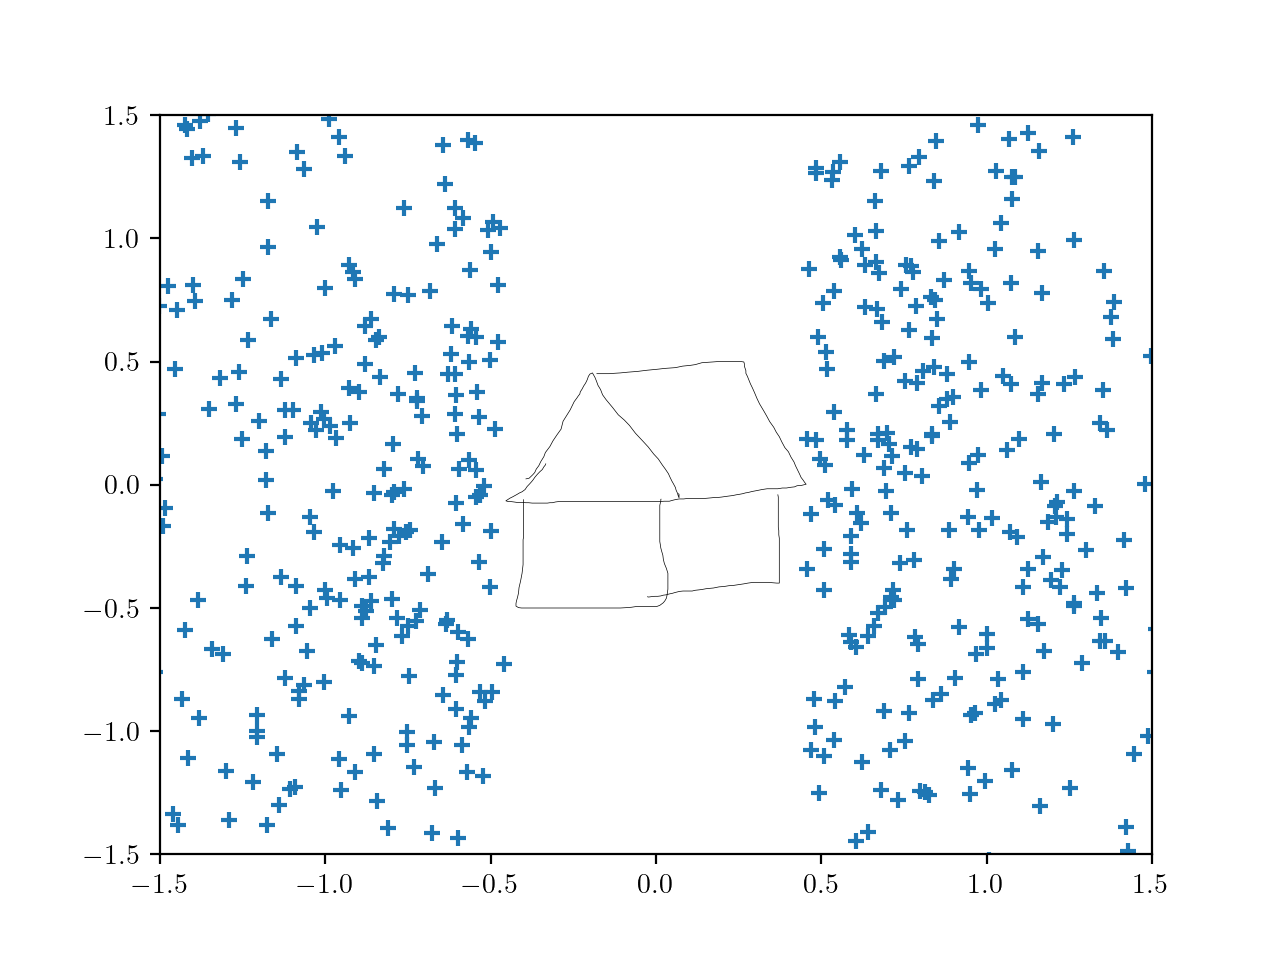
\includegraphics[width=\textwidth]{figures/rule_disjunct_side_house.png}
    \end{subfigure}
    \caption[Monte Carlo algorithm with rule-based constraints]{Monte Carlo algorithm finds points that satisfy given constraints. \emph{Inside} constraint on the left, \emph{side} constraint on the right.}
    \label{fig:monte_carlo:1}
\end{figure}

\subsection{Classifier-Based Constraints}
\label{sec:classifier_based_constraints}

The other approach uses a binary classifier trained on the \emph{Scene Graph} \citep{xu2017scenegraph}\break dataset. The classifier matches the constraint function definition \ref{constraint_function}. Given coordinates $(x, y)$, subject $a$, object $b$, and predicate $p$, the classifier decides whether the coordinates $(x, y)$ satisfy the constraint given by $a \xrightarrow{p} b$.

\begin{figure}[ht]
    \centering
    \begin{subfigure}{0.45\textwidth}
        \centering
        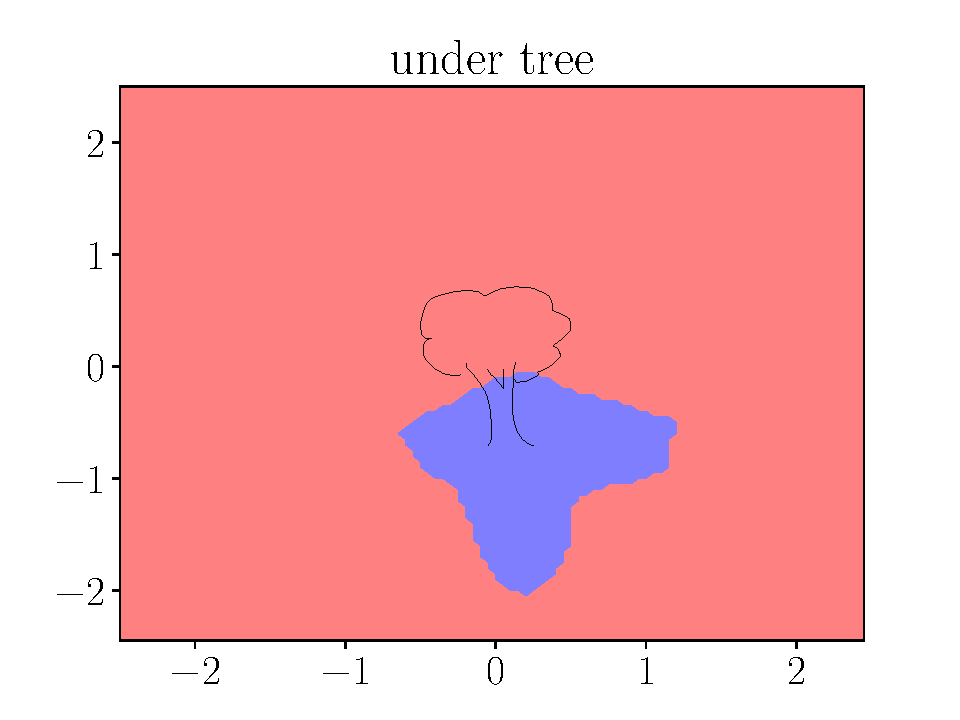
\includegraphics[width=\textwidth]{figures/under_tree}
    \end{subfigure}
    \begin{subfigure}{0.45\textwidth}
        \centering
        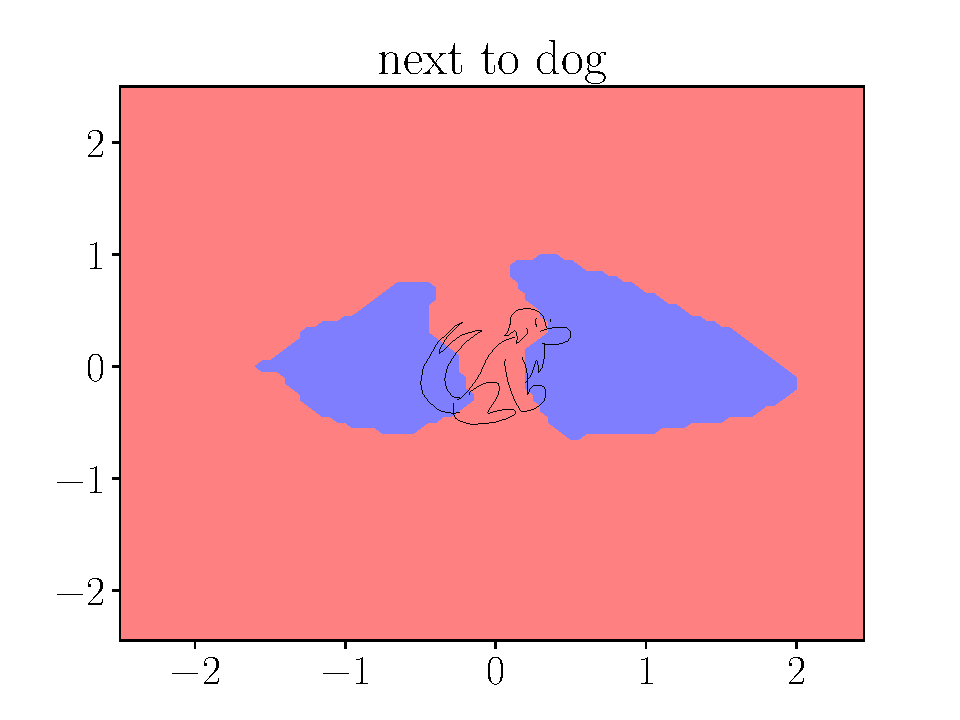
\includegraphics[width=\textwidth]{figures/next_to_dog}
    \end{subfigure}
    \caption[Visualisation of the classifier's decision boundaries]{Visualisation of the classifier's decision boundaries.}
    \label{fig:boundaries:1}
\end{figure}

\medskip

The classifier has four inputs -- subject, predicate, $x$ coordinate, and $y$ coordinate. The subject is encoded as a 100-dimensional vector using word embedding. The \emph{Scene Graph} dataset \citep{xu2017scenegraph} contains a limited number of predicates. We use the 50 most frequent ones; therefore, the predicate is encoded using a 50-dimensional one-hot vector. Each of the $x$ and $y$ coordinates is encoded as a single float number. Note that we use normalised coordinates relative to the centre of the subject -- the absolute $x$ and $y$ coordinates are converted to relative ones and divided by subjects' width and height, respectively.  In total, the classifier takes a 152-dimensional input. In \Cref{sec:constraint_results}, we also show results obtained with a classifier that only takes the predicates and the coordinates as inputs.

\medskip

The classifier itself is a multilayer perceptron with three hidden layers and a total of $600$ hidden units with ReLU activations. We use Stochastic Gradient Descent (SGD) as an optimiser and a cross-entropy loss.

\medskip

The source of the training data is the \emph{Scene Graph} dataset \citep{xu2017scenegraph}. The dataset contains the semantic subject-predicate-object triples as well as sizes and positions of the subjects and objects. The positions are absolute. We convert them to the relative position format described in the preceding sections. However, this dataset only contains correctly placed objects. To be able to train the classifier, we need to synthesise data that contains incorrectly placed objects. We do so by replacing the relative position of a subject-object-predicate triple with a position of another triple with a different predicate.

\subsection{Determining the Object's Size}
\label{sec:determining_obj_size}

Besides the object positions within a scene, we also need to determine their sizes. The \emph{Quick, Draw!} \citep{quickdraw} dataset contains $345$ categories. The relatively small number of categories makes it possible to define the absolute size for each category by hand. This is, in fact, our first approach for determining the object sizes. The objects in the scene can be scaled accordingly to the ratio between the defined sizes. In addition to the process being tedious, this approach also has one apparent flaw. The size ratio of objects often depends on context. For instance, the size ratio of a television and a car is different in the following sentences: \say{A car is on the television} and \say{The television is near the car.}.

\medskip

The mentioned problem of absolute sizes suggests a different approach. Instead of defining the absolute size for each category, we can define a relative size between a pair of categories. However, defining relative sizes for $119\,025$ pairs of categories by hand is infeasible. Instead, we once again use the \emph{Scene Graph} \citep{xu2017scenegraph} dataset to extract the relative sizes. The following list summarizes three methods used to determine the objects' sizes:
\begin{enumerate}
    \item Absolute -- For each \emph{Quick, Draw!} category, we extract absolute sizes of matching objects' bounding boxes from the dataset and use their average as a size.
    \item Relative -- If both subject and object are valid \emph{Quick, Draw!} categories, we compute the ratio of their widths and heights. We average these ratios across the whole dataset.
    \item Relative + word embedding -- Modification of the previous method where we do not require an exact match with a \emph{Quick, Draw!} category. Instead, we add the ratios to the most similar categories. The most similar categories are determined by the cosine similarity of their word embeddings. We also set different similarity thresholds. 
\end{enumerate}

Not all the \emph{Quick, Draw!} category pairs are present in the \emph{Scene Graph} dataset. To address this problem, the data obtained using the methods mentioned above can be completed by transitive closure. We estimate the unknown ratio $a:b$ between objects $a$ and $b$ as 
\begin{align*}
\frac{a}{b} = \frac{1}{n} \sum_{i = 0}^n \frac{a}{k_i} \cdot \frac{k_i}{b}
\end{align*}
where $a:k_i$ and $k_i:b$ are known ratios.

\section{Image Generation}

With a composed scene, the image generation itself is a straightforward process. Both position and size are known for all objects in the scene. The only thing left to do is to select a drawing of the object and draw it onto a drawing canvas. The drawings are randomly selected from the \emph{Quick, Draw!} \citep{quickdraw} dataset. We do not use the entire dataset as it also contains irrelevant and inappropriate data. Only a manually selected portion of the dataset is used.
